\subsection{Objective 1: \texttt{mpbenchmark}}
As mentioned in the introduction section \texttt{mpbenchmark} performs calculations of a jet engine using multiple threads and produces the time taken to complete these calculations as output. After analysing the code implementation of \texttt{mpbenchmark} the application can be summarised performing the following tasks:

\begin{enumerate}
	\item The application reads data from an input(\texttt{.txt}) file and stores that into an array before starting the calculations. This input data is required to perform calculations required in the next step. 
	\item During calculation, each thread reads input data at specific positions of the input array. After calculation, the results are written into an output array.
	\item In the last step, the benchmark’s response time along with deadlines missed is printed out and saved to an output(\texttt{.txt}) file. 
\end{enumerate}

This design of \texttt{mpbenchmark} can be visualised in figure \ref*{fig:revised_mpbenchmark_structure}.

\begin{figure}[h] % Positioning preference: here, top, bottom, page
	\centering
	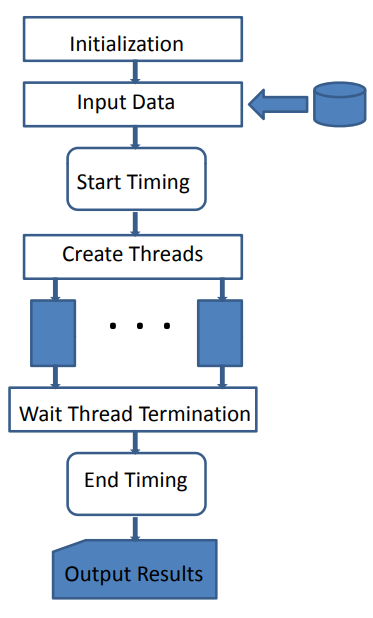
\includegraphics[width=0.5\textwidth, height=10cm]{~/Documents/Part_D_Modules/Individual_Project/Individual_report/figures/revised_mpbenchmark_structure.png} % Adjust the path and width as needed
	\caption{Revised \texttt{mpbenchmark} structure \cite{mpbenchmark_paper}.}
	\label{fig:revised_mpbenchmark_structure} % Use this label to reference the figure
\end{figure}

The source code of \texttt{mpbenchmark} provided a solution in \texttt{C\#}, this served as a useful reference of how figure \ref*{fig:revised_mpbenchmark_structure} would be implemented in code using object-oriented design. Subsequently, the \texttt{C++} object oriented design comprised of three main classes:

\begin{enumerate}
	\item \texttt{FileDataLoader}: the primary function of this class is to load data from the input file and also to allow the user to save output data to the output file.
	\item \texttt{SharedPerformanceData}: this class stores data loaded from the input file into an array and also allows storage of output data into a separate array. But importantly it allows threads to access specific parts of the input data in a thread-safe manner. 
	\item \texttt{Worker}: this class contains functions to perform the important calculations, computations of deadlines missed and output data. This class defines the \texttt{operator ()} which encapsulates the main calculations, this class design is know as a \texttt{Functor}.
\end{enumerate}

The \texttt{C++} object-oriented class design can be visualised using a UML class diagram [insert reference].

\subsection{Objective 2: \texttt{MobileNet}}
\subsection{Objective 3: \texttt{Debate-FI platform}}